\chapter{検証実験}\label{chap:experiment}

\section{概要}
本論文で提案する個人認証システムについて,3つの評価実験を行った.
それぞれの実験は,時間的な制約から予備実験,本実験などの形式で行うことをせず,一度に行った.

\subsection{実験手順}
以降の節のそれぞれの実験は第\ref{subsec:selectSecret}節にて挙げた3つの実装(以降,「パターン」と記載する)に対応しており,それぞれのパターンは多要素化手法として評価するために認証操作の後に4桁のPINによる認証操作を追加した.
そこに「PINの桁数を一桁増やし,5桁にしたものを秘密情報とする」パターンを追加し,計4パターンで相互に比較を行った.
各パターンの実験は一つにつき8日間にわたって実施,その間に設定した日から数えて,0日目(設定直後),1日目,3日目,8日目の4回の認証試行を行った.
それぞれのパターンで実験中の期間は重複せず,順番は偏りのないように設定し,そのスケジュールにそって全実験を実施した.
スケジュールは4つのパターンの組み合わせであり,その総数は$ {}_4 P _4 $の式で表される.
本実験ではこれら全てに固有の番号(以降,「スケジュール番号」と記載する)を付録\ref{apdx:schedule}の通り割り振って管理する.

\subsubsection{初回実験説明・導入}
\begin{enumerate}
  \item 実験担当者が実験の目的・注意事項・免責事項を説明する.この手順は付録\ref{apdx:experiment}の実験説明資料と操作説明資料を用いて行う.
  \item 不明な点があれば質問してもらう.
  \item 被験者のスケジュールを決定し,それに合わせて提案システムを実装したアプリケーションソフトウェア(以降「Notifauth」と記載する)のソースコードにスケジュール番号を登録する.
  \item 実験担当者の開発用端末と被験者の携帯端末を接続し,Appleの開発者用アカウントと被験者の端末の紐付けを行った上でNotifauthをインストールする.
  \item 実際にNotifauthを操作し,全てのパターンでひと通りの秘密情報設定と認証操作を行ってもらう.
  \item その後,Notifauth内の全ての保存されたデータを初期化し,スケジュールに沿ったパターンのみ設定を行ってもらうことで実験開始とする.
  \item 上記手順で設定したパターンについて認証操作を行ってもらう.
  \item この段階で実験データを送信してもらい,該当データの受信を実験担当者が確認ののち,初回実験説明・導入の終了とする.
\end{enumerate}

\subsubsection{試行手順}
\begin{enumerate}
  \item トップ画面で,試行したいパターンをセレクタで選択し,「Test」をタップする.
  \item ``PIN Mode''以外の場合,ロック画面を模した画面が表示され,秘密情報に当てはまると思われるツイートを見つけ,そのセルをスライドする.
  \item PINの入力画面が表示され,``PIN Mode''であれば5桁,それ以外のパターンであれば4桁のPINを入力する.
  \item 結果画面が表示されるので,「Home」をタップする.
\end{enumerate}

\subsubsection{結果送信手順}
\begin{enumerate}
  \item トップ画面で「Send」をタップすると,iOS標準のメール送信画面が開くので,何も編集を行わずに送信する.
  \item ここで仮にiOSへ自分のメール情報(送信サーバ,アカウントなど)が登録されていない場合以下の手順を行う
  \begin{enumerate}
    \item 「Send」をタップせず,トップ画面下部の「copy experiment data on clipboard」をタップする.
    \item クリップボードにデータがコピーされているので,メールアプリに貼り付けて実験担当者のメールアドレスへ送信する.
  \end{enumerate}
\end{enumerate}

\subsection{被験者}
男性12名,女性3名の計15名が実験を行った.
うち本学の学生は5名であった.
性別や年齢は表\ref{tab:participants}の通りである.
全ての検証実験を終了したのは12人で,そのうち最終アンケートに答えたのは○人である.
中間アンケートには○人が回答した.

\begin{table}[ht]
  \begin{minipage}{0.5\hsize}
    \begin{center}
      \small
      \begin{tabular}{l|r} \hline
        性別 \\ \hline
        男性 & 15 \\
        女性 & 3 \\ \hline
      \end{tabular}
    \end{center}
  \end{minipage}
  \begin{minipage}{0.5\hsize}
    \begin{center}
      \small
      \begin{tabular}{l|r} \hline
        年齢  \\ \hline
        10代 & 0 \\
        20代 & 12 \\
        30代 & 2 \\
        40代 & 1 \\
        50代以上 & 0 \\ \hline
      \end{tabular}
    \end{center}
  \end{minipage}
  \caption{被験者の特性}
  \label{tab:participants}
\end{table}

\section{SNSの情報を利用することに関する評価実験}\label{sec:vsTweet}
\subsection{目的}
本実験では,SNSの情報を利用することで,従来のPINを一桁増やした認証と比較し,どれだけ利便性と安全性を向上させることができるかの評価を行う.
本実験で評価対象とするパターンとして,``Manual Mode''を採用する.
アプリケーションを用いた実験では以下の3指標を測定する.

\begin{itemize}
  \item 短期の記憶保持
    \begin{description}
      \item[測定方法] 0日目,1日目,3日目の認証成功率を比較し,有意差をみる.
      \item[意義] 短期に記憶が保持できなければ,使用の継続が難しくなってしまうため.
      \item[目標] 5桁のPIN認証よりも平均での認証率が高く,日数によって認証成功率が落ちにくいことを目指す.
    \end{description}
  \item 長期の記憶保持
    \begin{description}
      \item[測定方法] 3日目と8日目の認証成功率を比較し,有意差をみる.
      \item[意義] 長期に記憶が保持できなければ,該当の認証を使わない期間が存在した際に認証できず,ユーザに秘密情報の再設定などの負担を与えてしまうため.
      \item[目標] 5桁のPIN認証よりも平均での認証率が高く,日数によって認証成功率が落ちにくいことを目指す.
    \end{description}
  \item 認証時間
    \begin{description}
      \item[測定方法] 認証操作の画面が表示されてから,認証を終えるまでの時間を計測する.認証の成否は問わないものとする.
      \item[意義] 認証操作に時間がかかりすぎてしまっては,携帯端末は一日に何度も認証を行うという仮定のもとでは,ユーザをいらいらさせてしまったりして,利便性を損ねてしまうため.
      \item[目標] 5桁のPIN認証よりも認証時間が短いことを目指す.
    \end{description}
\end{itemize}

\subsection{方法}
被験者実験により各試行の成功と失敗,認証にかかった時間を収集する.
また,付録の\ref{apdx:interimEnquete}や\ref{apdx:finalEnquete}にある通り,被験者には使用パターンについて5段階のリッカート尺度を使った質問に答えてもらい,さらに既に8日間の試行が終了している他パターンとの比較もしてもらう.

\subsection{結果}
本実験の結果を述べる.
試行のタイミングが1日程度前後した被験者が存在したため,1〜2日目を1日目,3〜6日目におこなったものを3日目,7〜8日目に行ったものを8日目の試行とした.
\begin{table}[ht]
  \begin{center}
    \small
    \begin{tabular}{|r|r|r|} \hline
      経過日数 & 認証成功率(\%) & 認証時間\\ \hline
      0 & 90.0 & 17.05 \\
      1~2 & 88.9 & 11.86 \\
      3~6 & 88.9 & 9.82 \\
      7~8 & 100.0 & 10.11 \\ \hline
    \end{tabular}
  \end{center}
  \caption{Manual Modeにおける各経過日数ごとの認証成功率と認証時間の変化}
  \label{tab:manual.data}
\end{table}

\begin{figure}[ht]
  \begin{center}
    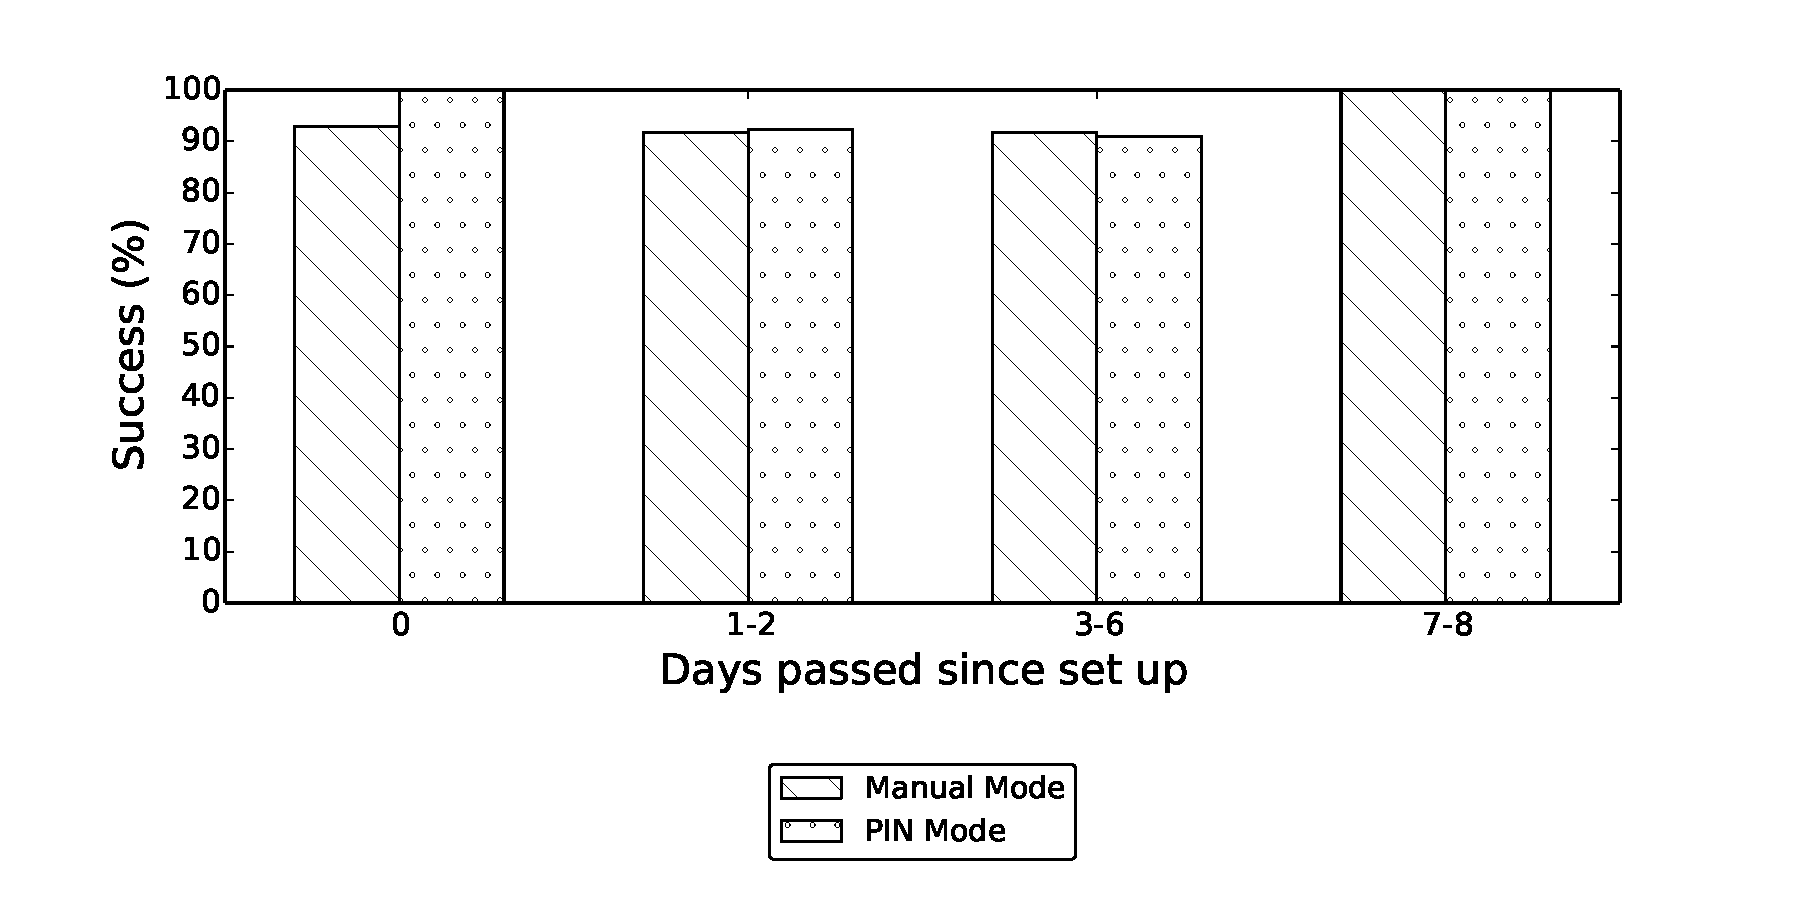
\epsfig{file=resource/ex_manual_vs_pin_rate.pdf,scale=0.5}
  \end{center}
  \caption{Manual ModeとPIN Modeにおける設定時からの経過日数ごとの認証成功率}
  \label{fig:ex_manual_vs_pin_rate}
\end{figure}

\begin{figure}[ht]
  \begin{center}
    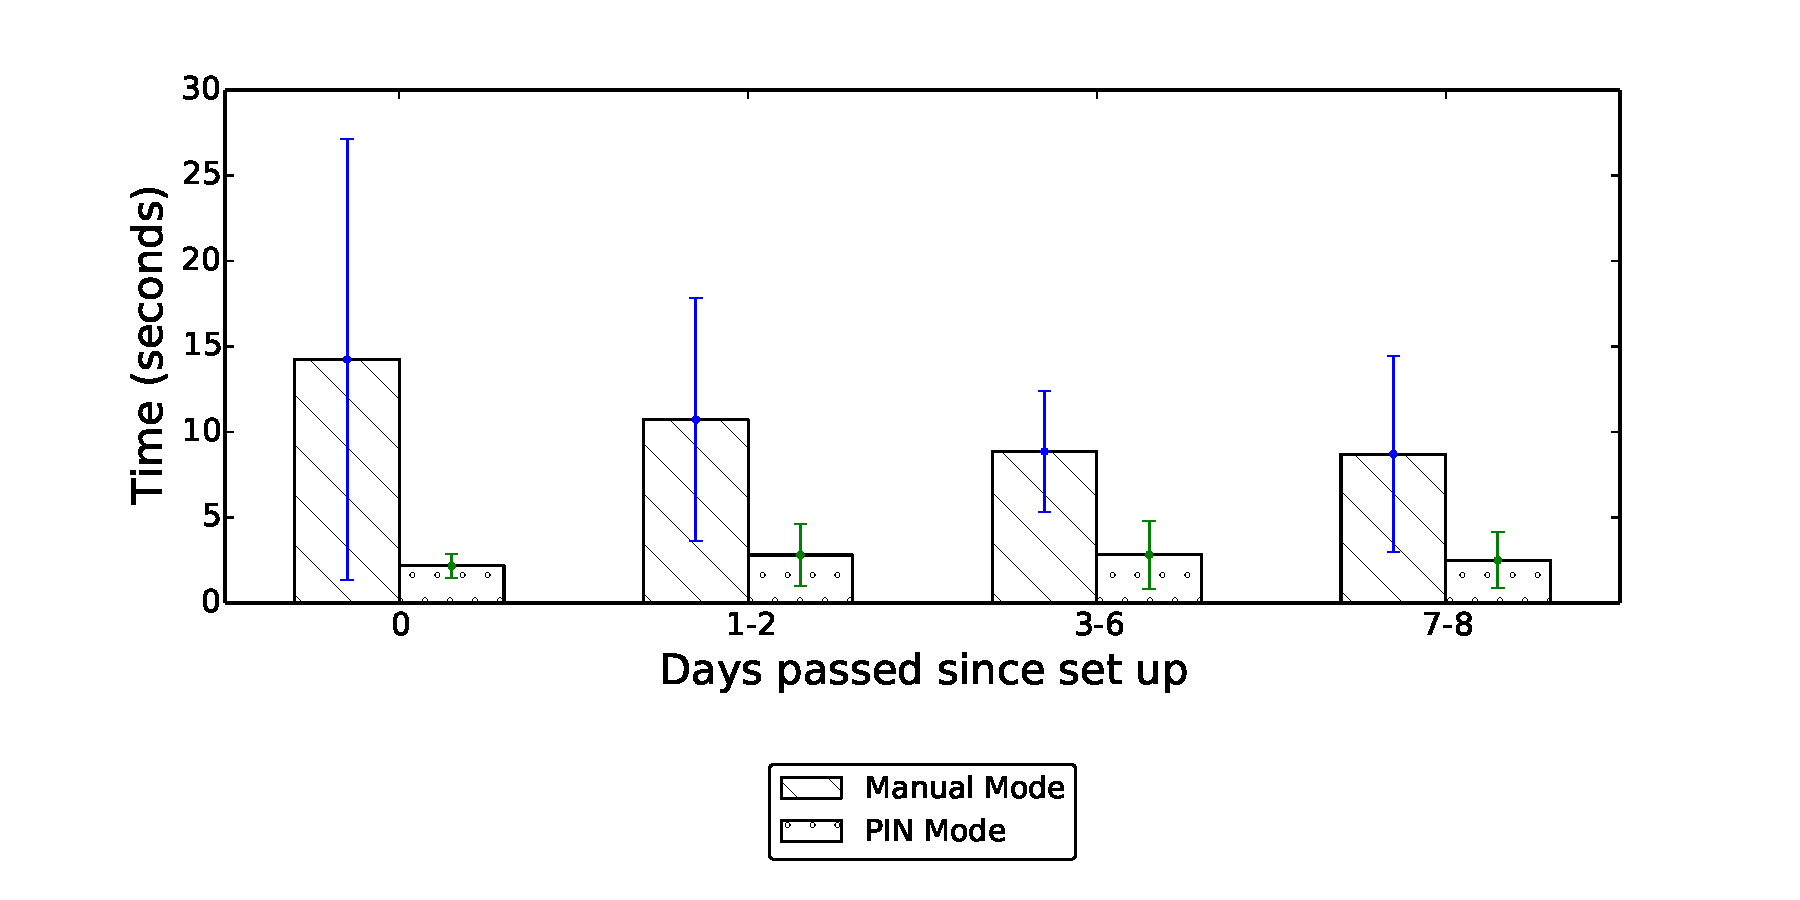
\epsfig{file=resource/ex_manual_vs_pin_time.pdf,scale=0.5}
  \end{center}
  \caption{Manual ModeとPIN Modeにおける設定時からの経過日数ごとの認証時間}
  \label{fig:ex_manual_vs_pin_time}
\end{figure}

\subsubsection{短期の記憶保持}


\subsubsection{長期の記憶保持}


\subsubsection{認証時間}


\section{時系列における期間を秘密として用いることに関する評価実験}\label{sec:vsTerm}
\subsection{目的}
本実験では,SNSの情報の特性を利用した認証システムの記憶持続性と利便性の評価を行う.
更に,ある一定のルールに基づいて秘密情報が変化することが認証の成功率やユーザへの負担がどう影響を与えるかについても検証する.
また,他の実験で用いたパターンとの比較も行う.
本実験で評価対象とするパターンとして,``Auto Mode Type Term''を採用する.
アプリケーションを用いた実験で測定した指標は第\ref{sec:vsTweet}節に準ずる.

\subsection{方法}
被験者実験により各試行の成功と失敗,認証にかかった時間を収集する.
また,付録の\ref{apdx:interimEnquete}や\ref{apdx:finalEnquete}にある通り,被験者には使用パターンについて5段階のリッカート尺度を使った質問に答えてもらい,さらに既に8日間の試行が終了している他パターンとの比較もしてもらう.

\subsection{結果}
本実験の結果を述べる.
試行のタイミングが1日程度前後した被験者が存在したため,1〜2日目を1日目,3〜6日目におこなったものを3日目,7〜8日目に行ったものを8日目の試行とした.
\begin{table}[ht]
  \begin{center}
    \small
    \begin{tabular}{|r|r|r|} \hline
      経過日数 & 認証成功率(\%) & 認証時間\\ \hline
      0 & 50.00 & 23.57 \\
      1〜2 & 42.86 & 18.65 \\
      3〜6 & 85.71 & 17.43 \\
      7〜8 & 66.67 & 14.74 \\ \hline
    \end{tabular}
  \end{center}
  \caption{Auto Mode Type Termにおける各経過日数ごとの認証成功率と認証時間の変化}
  \label{tab:auto_term.data}
\end{table}

\begin{figure}[ht]
  \begin{center}
    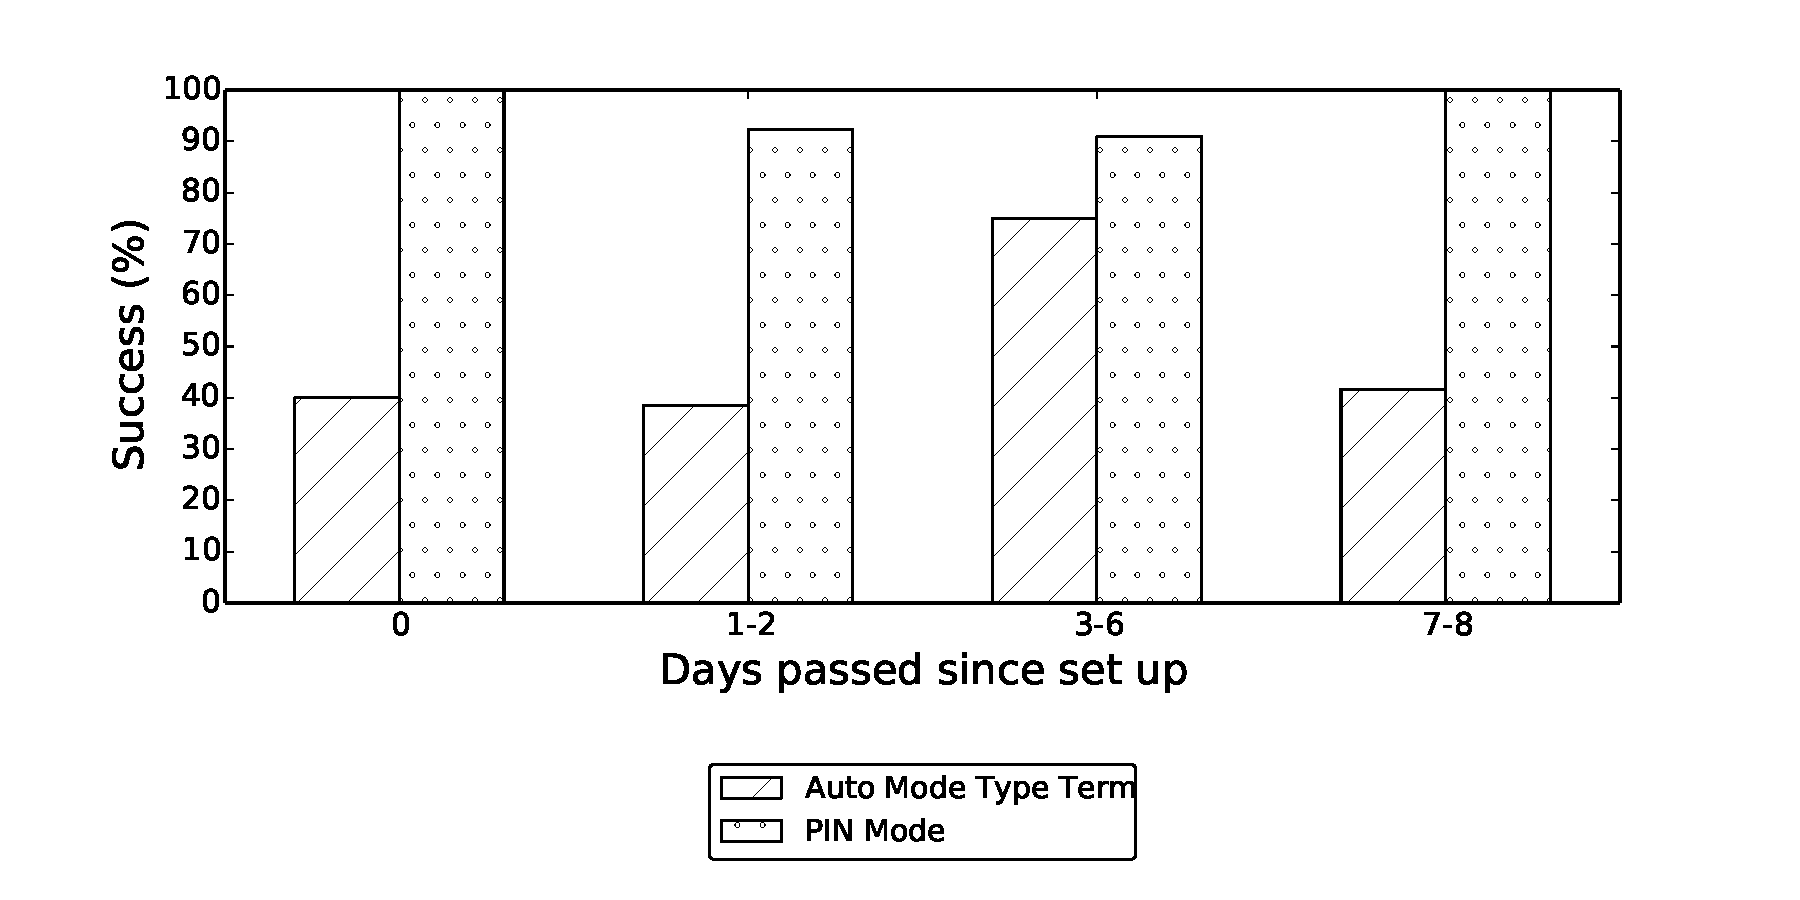
\epsfig{file=resource/ex_auto_term_vs_pin_rate.pdf,scale=0.5}
  \end{center}
  \caption{Auto Mode Type TermとPIN Modeにおける設定時からの経過日数ごとの認証成功率}
  \label{fig:ex_auto_term_vs_pin_rate}
\end{figure}

\begin{figure}[ht]
  \begin{center}
    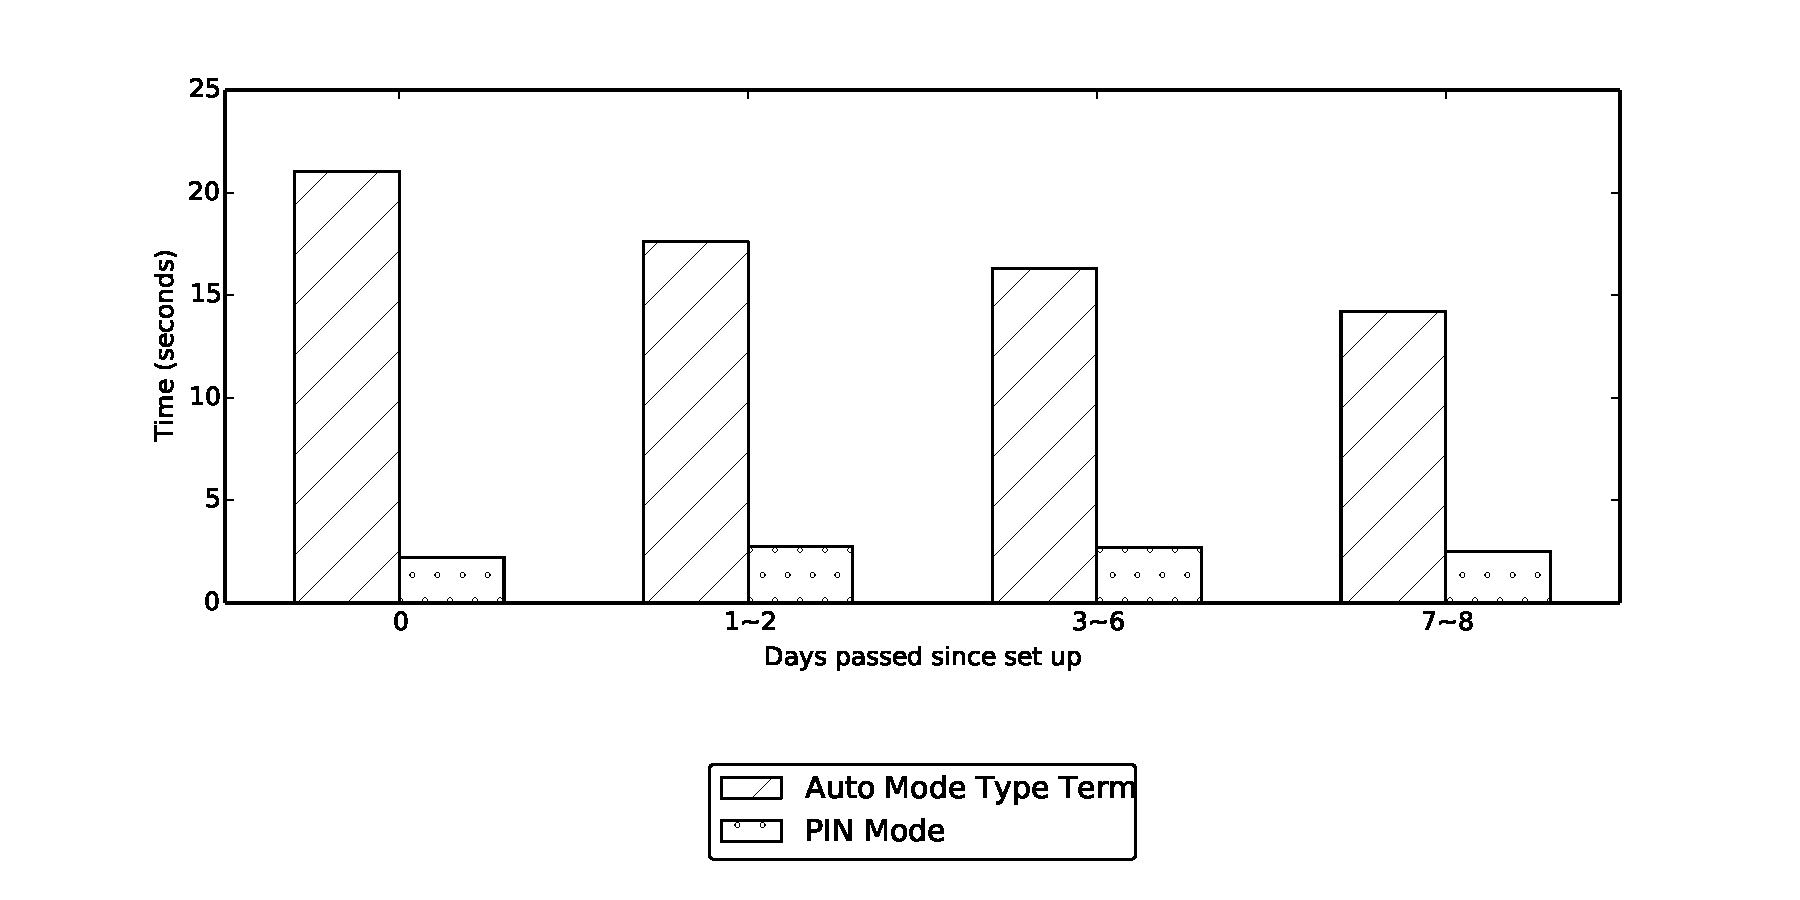
\epsfig{file=resource/ex_auto_term_vs_pin_time.pdf,scale=0.5}
  \end{center}
  \caption{Auto Mode Type TermとPIN Modeにおける設定時からの経過日数ごとの認証時間}
  \label{fig:ex_auto_term_vs_pin_time}
\end{figure}

\subsubsection{短期の記憶保持}


\subsubsection{長期の記憶保持}


\subsubsection{認証時間}


\section{時系列における周期を秘密として用いることに関する評価実験}\label{sec:vsCycle}
\subsection{目的}
本実験では,SNSの情報の特性を利用した認証システムの記憶持続性と利便性の評価を行う.
更に,ある一定のルールに基づいて秘密情報が変化することが認証の成功率やユーザへの負担がどう影響を与えるかについても検証する.
また,他の実験で用いたパターンとの比較も行う.
本実験で評価対象とするパターンとして,``Auto Mode Type Cycle''を採用する.
アプリケーションを用いた実験で測定した指標は第\ref{sec:vsTweet}節に準ずる.

\subsection{方法}
被験者実験により各試行の成功と失敗,認証にかかった時間を収集する.
また,付録の\ref{apdx:interimEnquete}や\ref{apdx:finalEnquete}にある通り,被験者には使用パターンについて5段階のリッカート尺度を使った質問に答えてもらい,さらに既に8日間の試行が終了している他パターンとの比較もしてもらう.

\subsection{結果}
本実験の結果を述べる.
試行のタイミングが1日程度前後した被験者が存在したため,1〜2日目を1日目,3〜6日目におこなったものを3日目,7〜8日目に行ったものを8日目の試行とした.
\begin{table}[ht]
  \begin{center}
    \small
    \begin{tabular}{|r|r|r|} \hline
      経過日数 & 認証成功率(\%) & 認証時間\\ \hline
      0 & 33.33 & 20.84 \\
      1〜2 & 20.00 & 20.42 \\
      3〜6 & 0.00 & 36.56 \\
      7〜8 & 16.67 & 24.19 \\ \hline
    \end{tabular}
  \end{center}
  \caption{Auto Mode Type Cycleにおける各経過日数ごとの認証成功率と認証時間の変化}
  \label{tab:auto_cycle.data}
\end{table}

\begin{figure}[ht]
  \begin{center}
    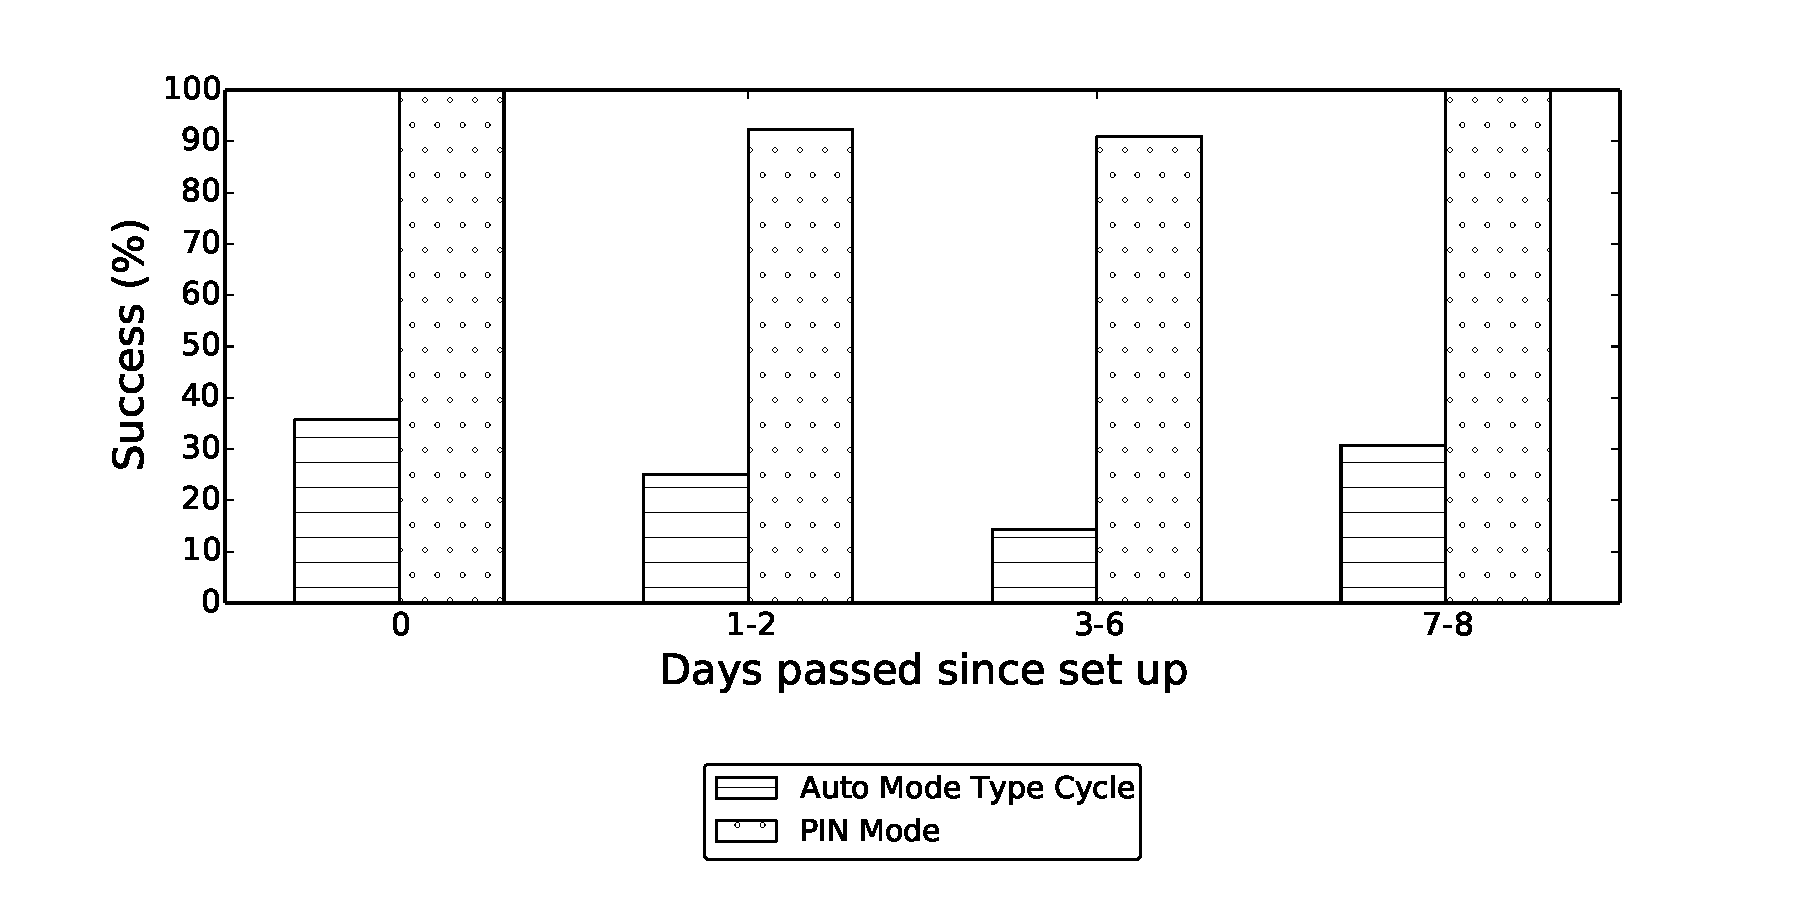
\epsfig{file=resource/ex_auto_cycle_vs_pin_rate.pdf,scale=0.5}
  \end{center}
  \caption{Auto Mode Type CycleとPIN Modeにおける設定時からの経過日数ごとの認証成功率}
  \label{fig:ex_auto_cycle_vs_pin_rate}
\end{figure}

\begin{figure}[ht]
  \begin{center}
    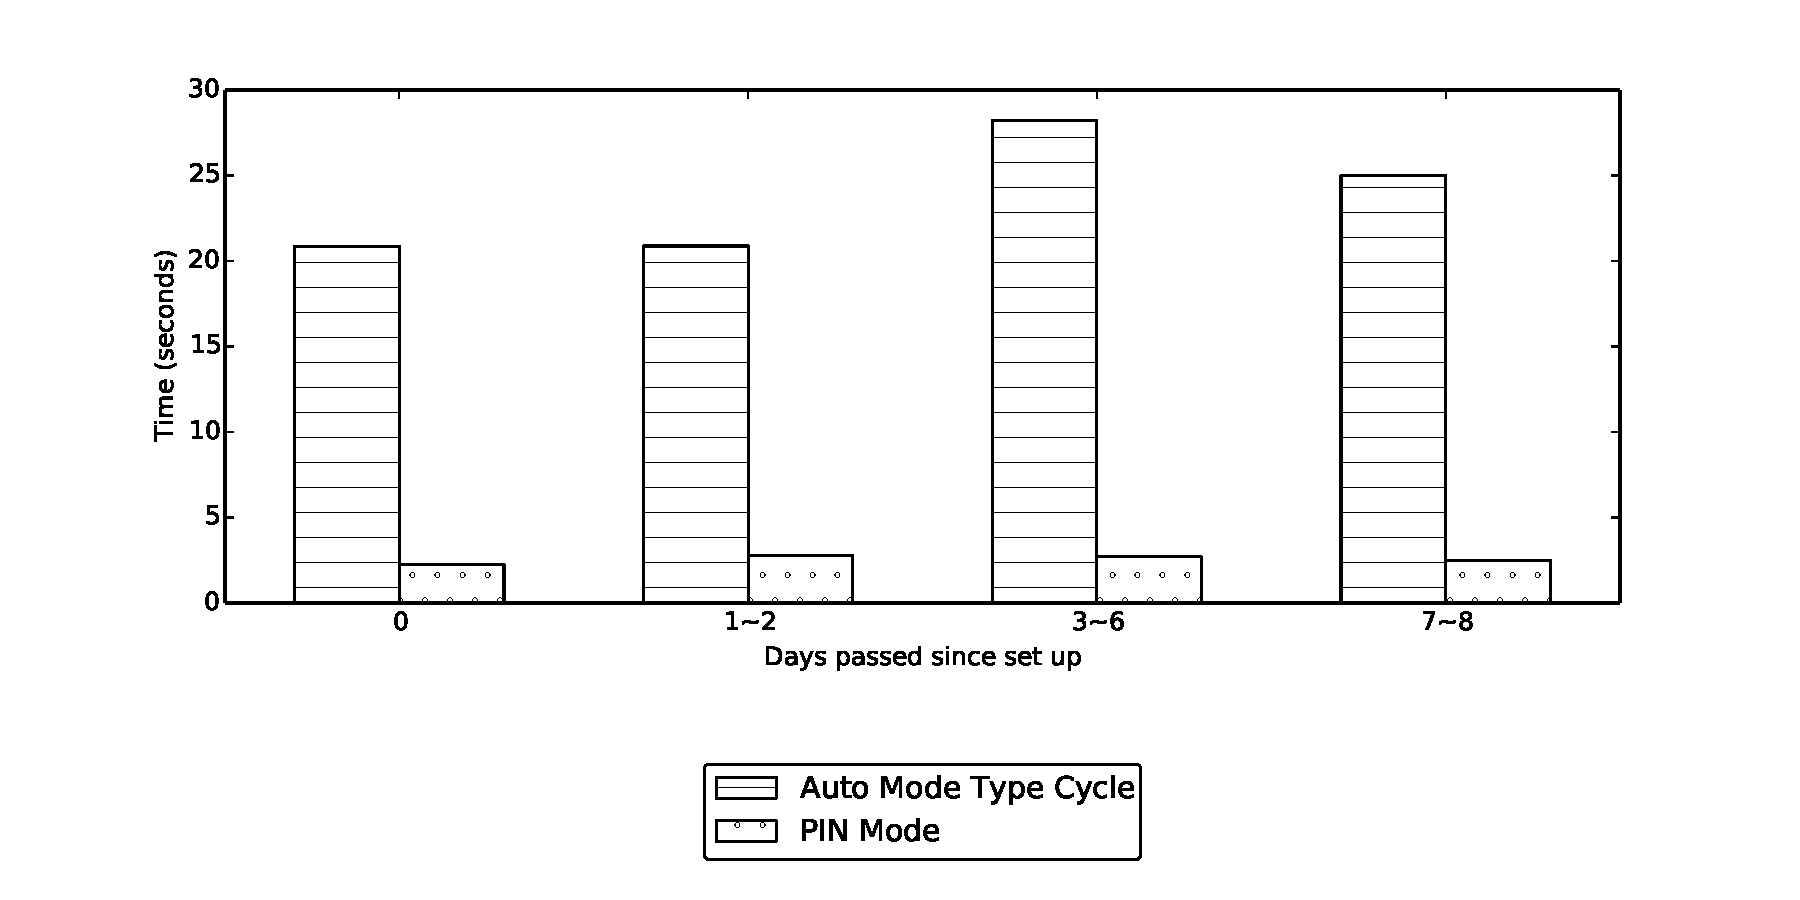
\epsfig{file=resource/ex_auto_cycle_vs_pin_time.pdf,scale=0.5}
  \end{center}
  \caption{Auto Mode Type CycleとPIN Modeにおける設定時からの経過日数ごとの認証時間}
  \label{fig:ex_auto_cycle_vs_pin_time}
\end{figure}

\subsubsection{短期の記憶保持}


\subsubsection{長期の記憶保持}


\subsubsection{認証時間}



\section{各評価実験での相互比較}\label{sec:vsAll}
\subsection{目的}
本節では,各評価実験で行ったパターン全てのなかで比較を行う.

\subsection{方法}
被験者実験により各試行の成功と失敗,認証にかかった時間を収集する.
また,付録の\ref{apdx:interimEnquete}や\ref{apdx:finalEnquete}にある通り,被験者には使用パターンについて5段階のリッカート尺度を使った質問に答えてもらい,さらに既に8日間の試行が終了している他パターンとの比較もしてもらう.

\subsection{結果}


\newpage

